\clearpage
\chapter{Results}\label{chap:results}

Well over 1 billion games were simulated in the process of evaluating the
chromosomes in this experiment. One thousand generations were evolved for every
combination of population size (32, 128, 512, and 1024), chromosome type (RGA,
SGA, and TGA), number of games played by each chromosome in a generation (7, 25,
50, 100), and fitness evaluator (FINISH\_ORDER, NET\_WORTH, NUM\_MONOPOLIES,
NUM\_PROPERTIES, NUM\_WINS, and TOURNAMENT\footnote{For the tournament fitness
evaluator the number of games was determined by the population size and was not
independent. So for TOURNAMENT, 1000 generations were evolved for every
combination of population size and chromosome type}). Results of the
evolutionary process are presented in the first section of this Chapter.

In the first section, results for the RGA chromosome are presented first, and in
a large amount detail. We also look briefly at the results for the SGA
chromosomes, even though players with this chromosome tended to evolve poorly.
This is most likely due to the fact that the data structure used for the SGA
chromosomes is not well suited to the problem domain. Finally, results for the
TGA chromosomes are also briefly discussed, but these players were almost
identical to the RGA chromosomes and so do not provide much of any additional
insight. Because the evolution of SGA and TGA chromosomes do not provide any
useful information, the remainder of the chapter focuses exclusively on results
obtained from the RGA chromosomes.

After the evolutionary process was complete, the best players from each
generation were competed in various combinations to validate the results. 

First, an intra-population validation was performed where the best players from
different generations within a population were competed against each other. For
most populations, players in later generations were better than players in
earlier generations, which suggests that the genetic algorithm was successful in
evolving players. We will also show that populations that play more games per
generation tended to evolve better players than populations with less games per
generation. 

Second, players were also validated with an inter-population validation. That
is, the best players from different populations were competed against each other
in various combinations. Since the first analysis showed that populations that
played more games per generation tended to evolve better players, only players
from the populations that played 100 games per generation were
competed\footnote{Except for TOURNAMENT in which the most games per generation
was 9, for the population size 1024.}. In this validation, various fitness
evaluators were compared to see which fitness evaluator evolved the best
players.

Finally, different population sizes are compared. In this validation, we expect
that players from larger populations would tend to evolve into better players.
The validation shows that this expectation was correct.

The results from the intra- and inter-population competitions are discussed in
the second section of this Chapter.

In the last section of this Chapter, results from real-world competitions are
presented. Based on the previous intra- and inter-population validations
performed, a set of the best overall players that evolved were selected and then
competed against human players and AI players available online.

\section{The evolutionary process and its results}

In a genetic algorithm which can use an objective fitness function, we expect
that the initial population has fitness values which are uniformly distributed.
In other words, the probability of an individual having average fitness is the
same as the probability of having low fitness or high fitness. As the population
is evolved, average fitness should steadily improve until a plateau is reached,
and the average error should decrease to some minimal value.

The expected results for for a competitive fitness function are different. Since
the first generation is randomly created, it is expected that the players will
be randomly spread in their ability to win games. Some players will win games,
some will lose games, and the average player will win about half the games they
play. So the probability that an individual has average fitness is higher than
the probability that an individuals has low or high fitness. The distribution of
fitness scores should follow a distribution similar to the binomial distribution
(See Figure~\ref{figure-binomial}).

\begin{figure}[htbp]
\centerline{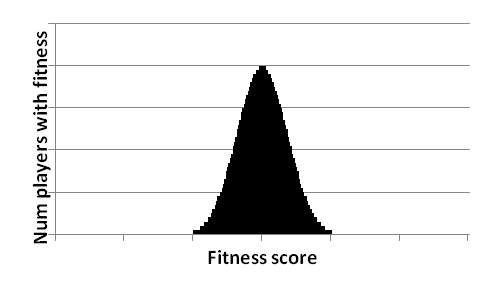
\includegraphics[width=0.75\columnwidth]{Figures/binomial.png}}
\caption[Binomial Distribution]{The expected fitness distribution for the first
generation of a population. A peak is expected around the average population
fitness. The distribution is similar to a binomial distribution.}
\label{figure-binomial}
\end{figure}

\subsection{Results for Initial Generations}

When the initial population of players was run through a single generation, the
actual results matched the expected results quite closely. 

For example, it can clearly be seen that the fitness distribution looks like a
binomial distribution when the FINISH\_ORDER fitness evaluator is used.
Figure~\ref{figure-RGA-G000-N100-FO-initial_fitness} shows the fitness
distribution for the first generation of an RGA population with the
FINISH\_ORDER fitness evaluator. The figure shows a binomial shaped distribution
which appears to be centered around the population average of 150. Because the
FINISH\_ORDER evaluator assigns 1, 2, and 3 points to the players in a game, for
a total of 6 points per game, the average fitness for any single game is \(6/4\)
or 1.5. So for \(n\) games the average fitness is \(n * 1.5\).
For a population that plays 100 games per generation, we expect that the fitness
scores in any generation will have a distribution that is centered on the
average score of 150.

\begin{figure}[htbp]
\centerline{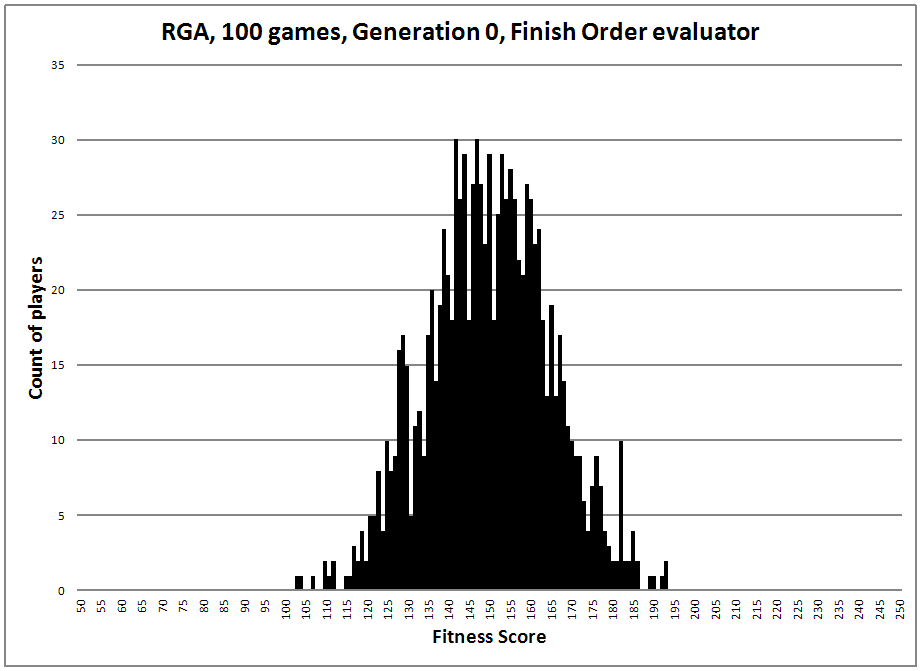
\includegraphics[width=0.75\columnwidth]{Figures/RGA_1024_G000_N100_FO.png}}
\caption[RGA Fitness Distribution, Initial Generation]{RGA chromosome,
generation 0, 100 games per generation, finish order fitness evaluator.}
\label{figure-RGA-G000-N100-FO-initial_fitness}
\end{figure}

% This same process (initialize a population and compete for a single generation)
% was repeated for thirty trials. This was done for all the various combinations
% of parameters.

The NUM\_WINS fitness evaluator is similar to FINISH\_ORDER. Every game will
always award 3 points to the winner, so the average fitness for a single game is
\(3/4\) or 0.75. So for \(n\) games the average fitness is \(n * 1.5\).
Figure~\ref{figure-RGA-G000-N100-NW-initial_fitness} shows the fitness
distribution for the first generation of an RGA population with the
NUM\_WINS fitness evaluator. The figure shows a binomial shaped distribution
which appears to be centered around the population average of 75.

\begin{figure}[htbp]
\centerline{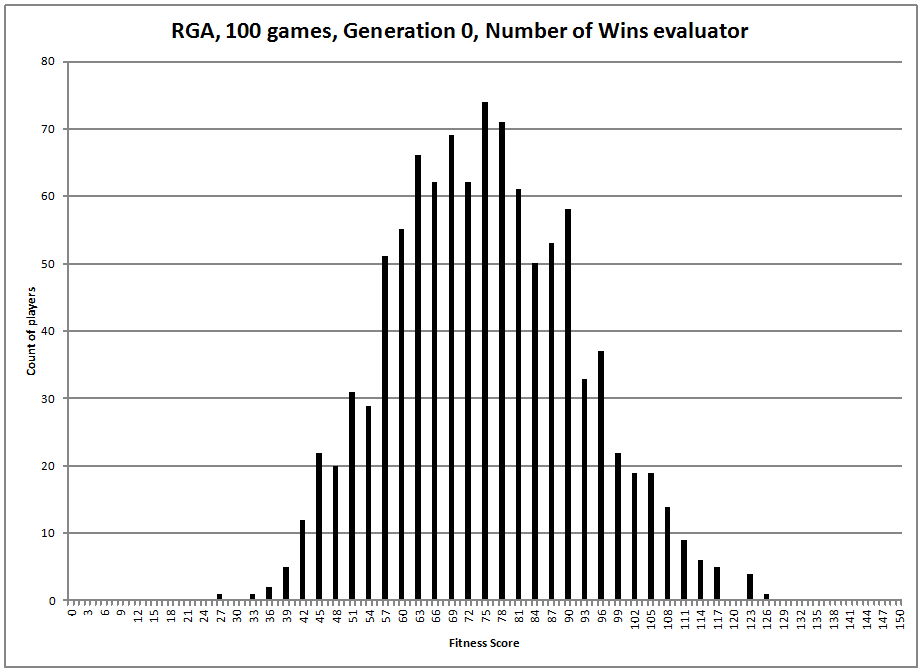
\includegraphics[width=0.75\columnwidth]{Figures/RGA_1024_G000_N100_NW.png}}
\caption[RGA Fitness Distribution, Initial Generation]{RGA chromosome,
generation 0, 100 games per generation, number of wins fitness evaluator.}
\label{figure-RGA-G000-N100-NW-initial_fitness}
\end{figure}

The fitness distribution for the initial generation with the NET\_WORTH fitness
evaluator is shown in Figure~\ref{figure-RGA-G000-N100-NetW-initial_fitness}.
The fitness distribution for the initial generation with the NUM\_MONOPOLIES
fitness evaluator is shown in
Figure~\ref{figure-RGA-G000-N100-NM-initial_fitness}.
The fitness distributions for the initial generation with the NUM\_PROPERTIES
fitness evaluator is shown in
Figure~\ref{figure-RGA-G000-N100-NP-initial_fitness}.

\begin{figure}[htbp]
\centerline{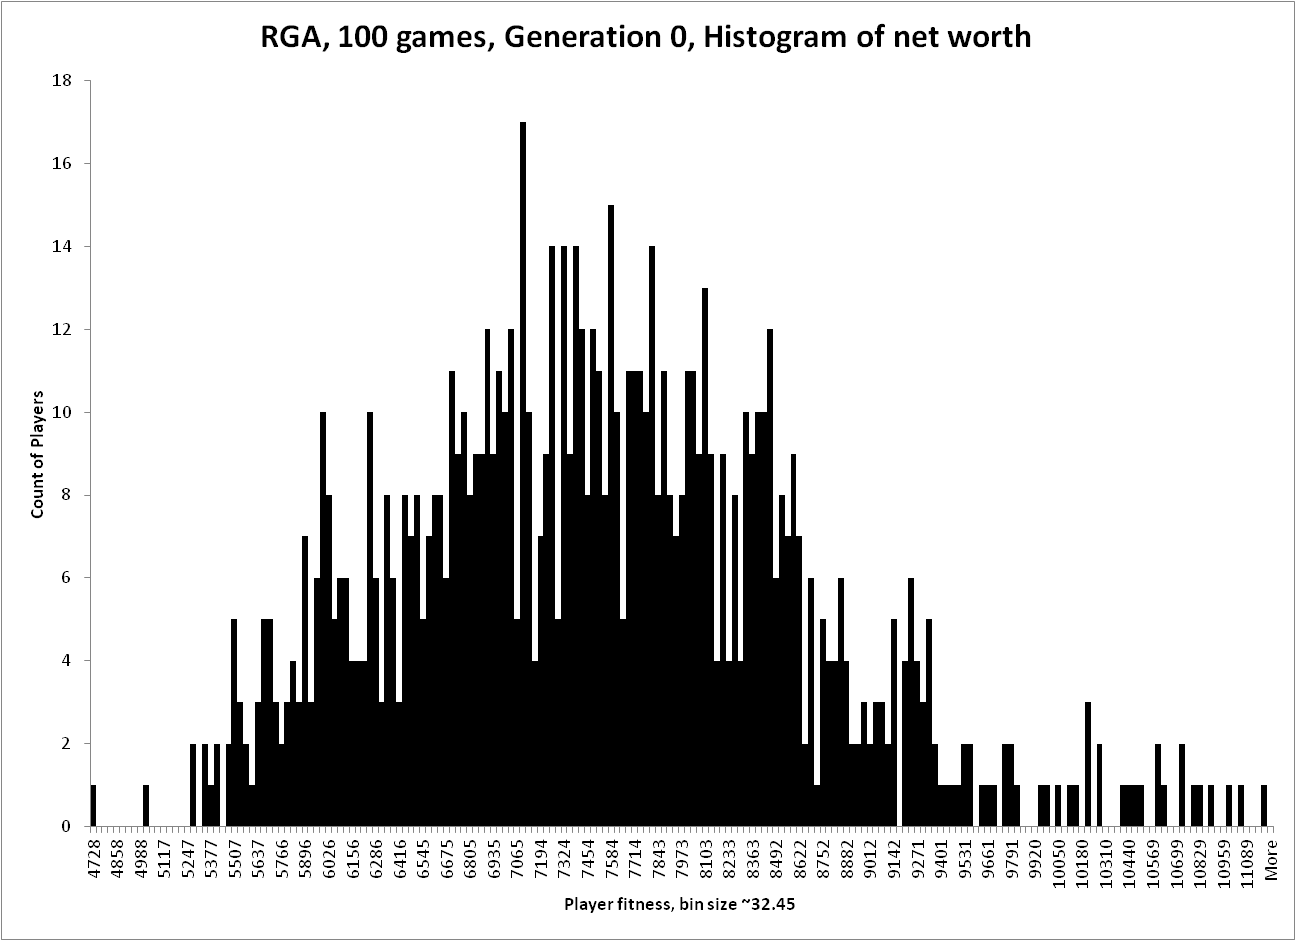
\includegraphics[width=0.75\columnwidth]{Figures/RGA_1024_G000_N100_NetW.png}}
\caption[RGA Fitness Distribution, Initial Generation]{RGA chromosome,
generation 0, 100 games per generation, net worth fitness evaluator.}
\label{figure-RGA-G000-N100-NetW-initial_fitness}
\end{figure}

\begin{figure}[htbp]
\centerline{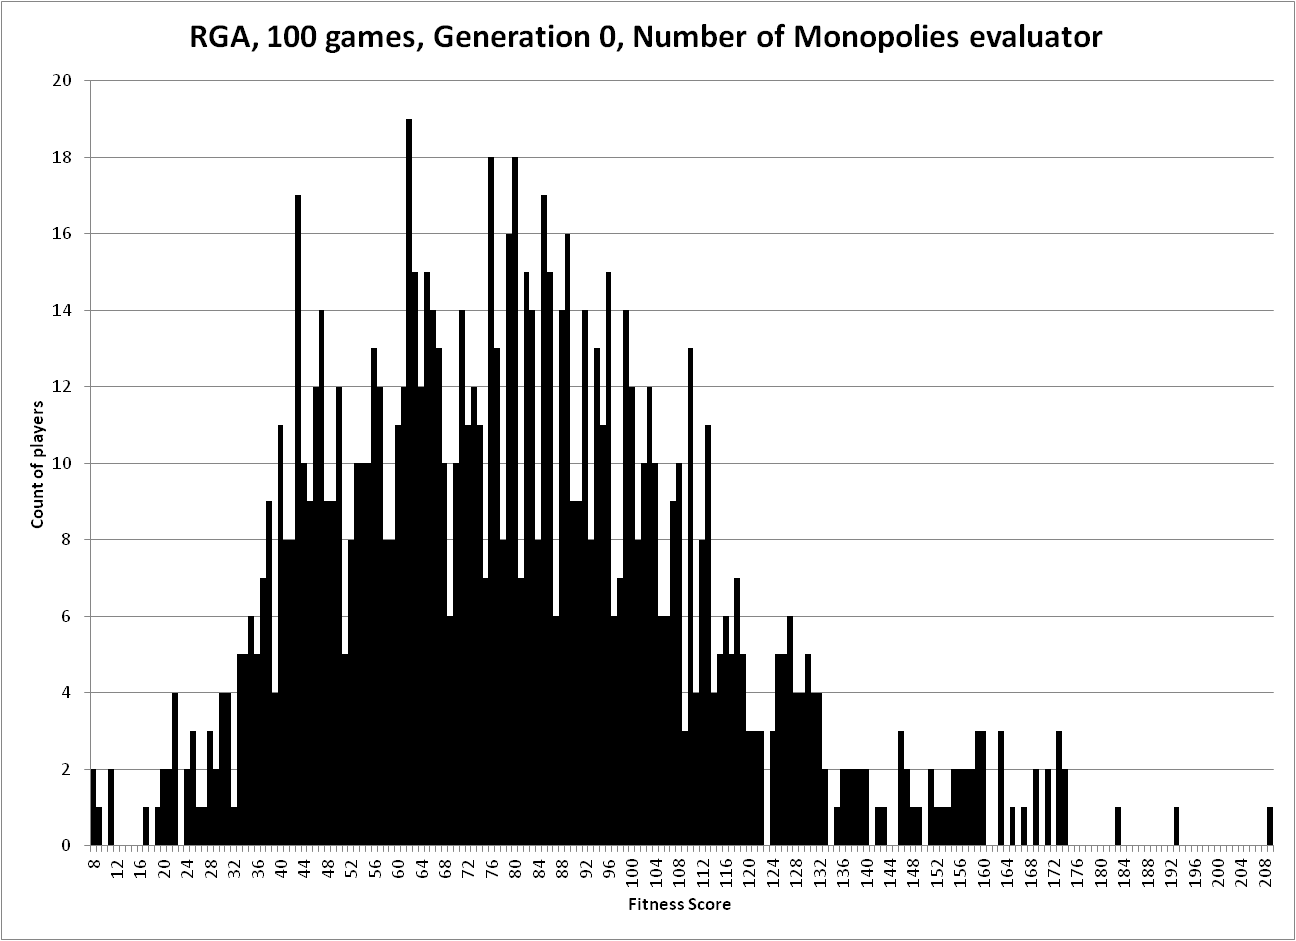
\includegraphics[width=0.75\columnwidth]{Figures/RGA_1024_G000_N100_NM.png}}
\caption[RGA Fitness Distribution, Initial Generation]{RGA chromosome,
generation 0, 100 games per generation, number of monopolies evaluator.}
\label{figure-RGA-G000-N100-NM-initial_fitness}
\end{figure}

\begin{figure}[htbp]
\centerline{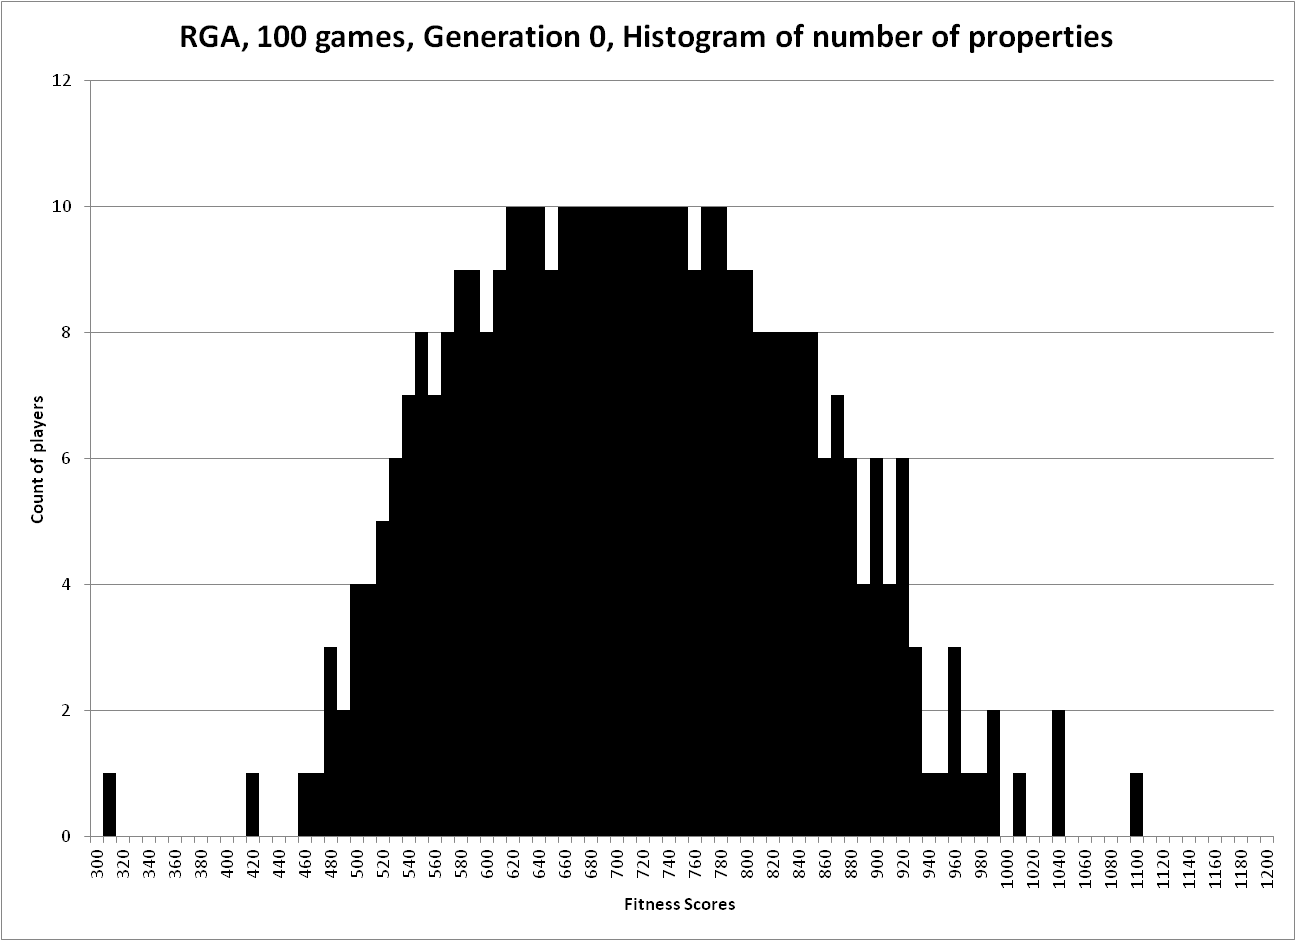
\includegraphics[width=0.75\columnwidth]{Figures/RGA_1024_G000_N100_NP.png}}
\caption[RGA Fitness Distribution, Initial Generation]{RGA chromosome,
generation 0, 100 games per generation, number of properties fitness evaluator.}
\label{figure-RGA-G000-N100-NP-initial_fitness}
\end{figure}

\subsection{Results for Subsequent Generations}

The other difference between a competitive fitness function and an objective
fitness function is that as the population co-evolves under a competitive
fitness function the average and best fitness scores are not expected to
increase. Rather the average fitness will remain the same as the initial
population, and the worst and best fitness scores should tend to converge
towards the average. As the players get better and the population is more evenly
matched, most players will tend to win half the games they play.

This is because the fitness is measured by awarding points to players as they
play against each other in games. So, as poor players are removed from the
population, the remaining players will tend to be near each other in
``ability.'' Thus, the distribution of fitness scores will become much tighter
around the average score, and no single player will be able to dominate the
other players.

Figure~\ref{figure-100th_gen_fitness} shows the actual fitness distribution at
generation 100 of an RGA population with the FINISH\_ORDER fitness evaluator. As
predicted, it can be seen that the mean remained approximately the same, but the
variance has appeared to decrease. Whereas the fitness scores in generation 0
ranged from 103 to 193, in generation 100 they ranged from 115 to 186. The
distribution around the mean tightened relatively quickly (it can clearly be
seen in generation 100), and then remained fairly constant over the course of
the simulation which was 1000 generations.

\begin{figure}[htp]
\centerline{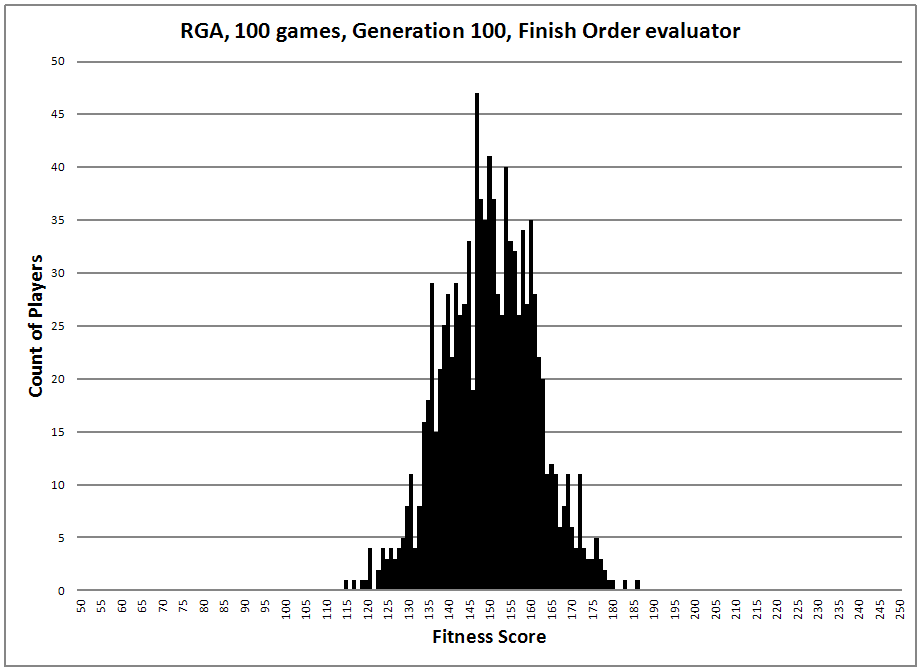
\includegraphics[width=0.75\columnwidth]{Figures/RGA_1024_G100_N100_FO.png}}
\caption[RGA Fitness Distribution, 100th Generation]{RGA chromosome, generation
100, 100 games per generation, finish order fitness evaluator.}
\label{figure-100th_gen_fitness}
\end{figure}

Additional plots of the distribution of fitness scores can be seen in
Figure~\ref{figure-RGA-250th_gen_fitness},
Figure~\ref{figure-RGA-500th_gen_fitness},
Figure~\ref{figure-RGA-750th_gen_fitness}, and
Figure~\ref{figure-RGA-999th_gen_fitness}. Each of these figures shows the same
population at various points in the evolution process. The size of the
population is 1024 individuals with an RGA chromosome. Each individual played
100 games in each generation (K-Random Opponents with \(K\approx300\). The
fitness evaluator is the FINISH\_ORDER evaluator.

\begin{figure}
\centering
%%----start of first figure----
\begin{minipage}[t]{0.47\linewidth}
\centering
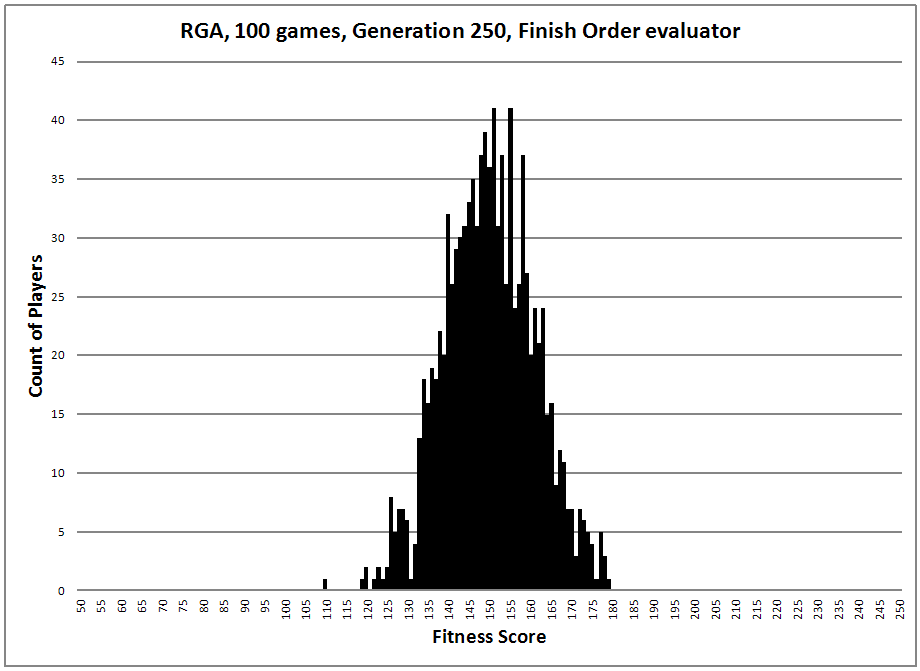
\includegraphics[width=1.0\linewidth]{Figures/RGA_1024_G250_N100_FO.png}
\caption[RGA Fitness Distribution, 250th Generation]{RGA chromosome, generation
250, 100 games per generation, finish order fitness evaluator.} \label{figure-RGA-250th_gen_fitness}
\end{minipage}%
\hspace{0.06\linewidth}%
%%----start of second figure----
\begin{minipage}[t]{0.47\linewidth}
\centering
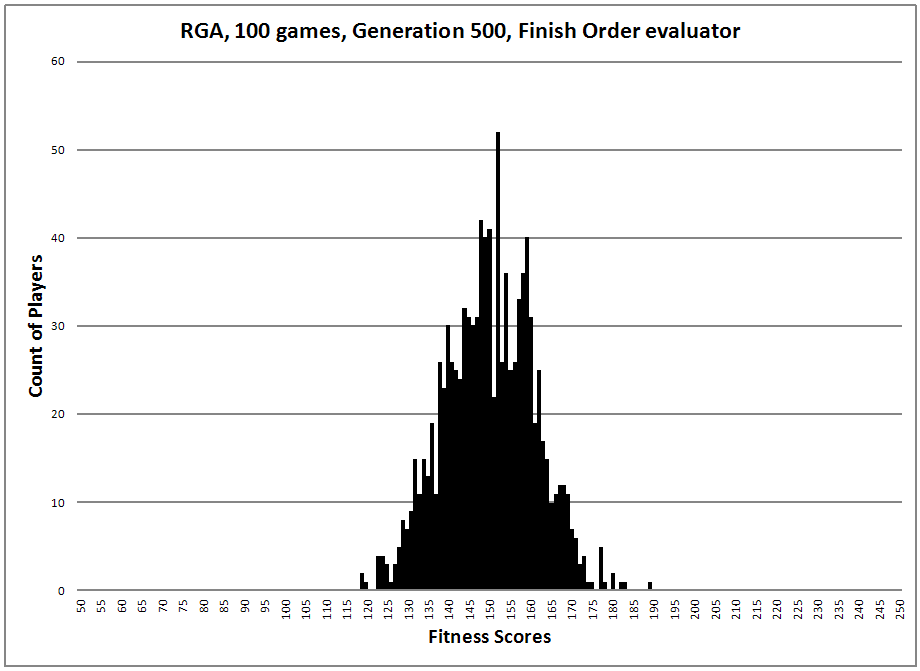
\includegraphics[width=1.0\linewidth]{Figures/RGA_1024_G500_N100_FO.png}
\caption[RGA Fitness Distribution, 500th Generation]{RGA chromosome, generation
500, 100 games per generation, finish order fitness evaluator.} \label{figure-RGA-500th_gen_fitness}
\end{minipage}
\\[\intextsep]

\begin{minipage}[t]{0.47\linewidth}
\centering
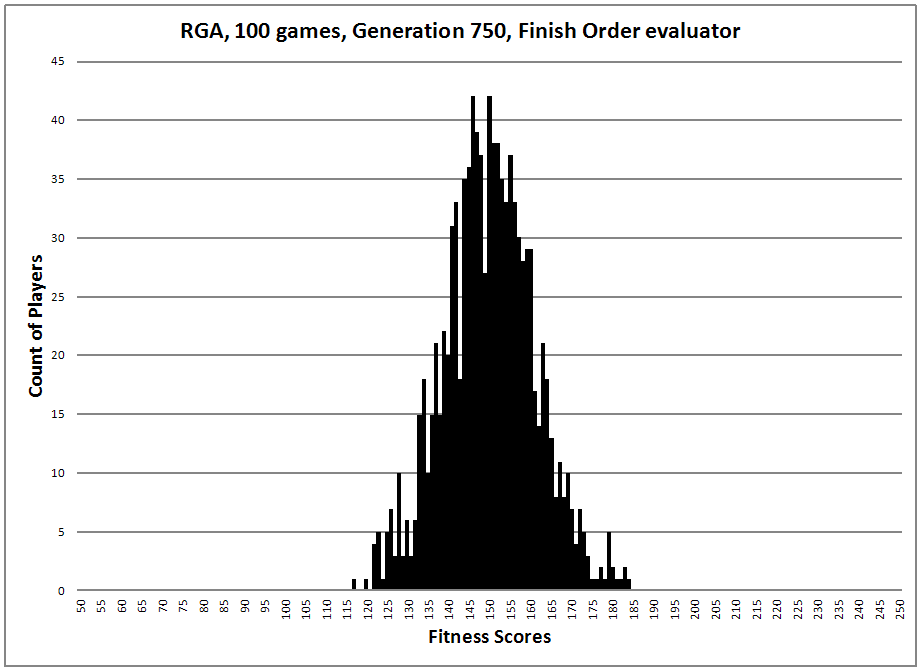
\includegraphics[width=1.0\linewidth]{Figures/RGA_1024_G750_N100_FO.png}
\caption[RGA Fitness Distribution, 750th Generation]{RGA chromosome, generation
750, 100 games per generation, finish order fitness evaluator.} \label{figure-RGA-750th_gen_fitness}
\end{minipage}%
\hspace{0.06\linewidth}%
%%----start of second figure----
\begin{minipage}[t]{0.47\linewidth}
\centering
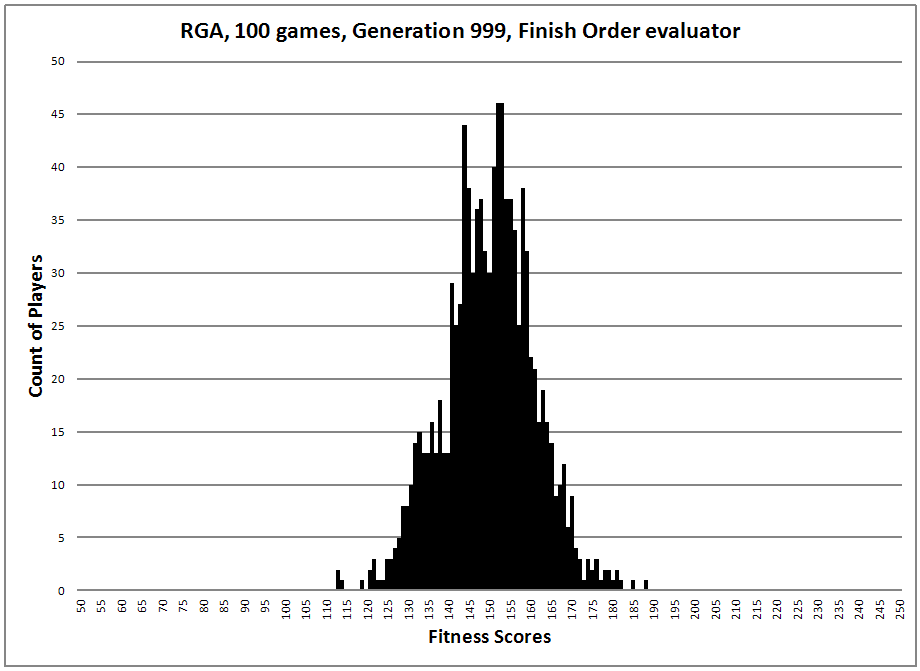
\includegraphics[width=1.0\linewidth]{Figures/RGA_1024_G999_N100_FO.png}
\caption[RGA Fitness Distribution, 999th Generation]{RGA chromosome, generation
999, 100 games per generation, finish order fitness evaluator.} \label{figure-RGA-999th_gen_fitness}

\end{minipage}
\end{figure}

Inspecting Figures~\ref{figure-RGA-250th_gen_fitness} through
\ref{figure-RGA-999th_gen_fitness}, it appears that at some point between the
100th generation and the 250th generation~\footnote{Because of the large amount
of data generated by the simulations, data for every generation was not output
by the simulation. Instead fitness data was output and saved for the initial
population, the 100th generation, and every 250th generation. Thus, the point at
which the population average fitness reaches the plateau cannot be calculated.
However, in a coevolutionary environment this is not a problem. A coevolutionary
population can continue to improve even though the fitness appears to plateau.
This will be further discussed later in this Chapter.}, that the population
average fitness reaches a plateau. This is also demonstrated by looking at some
of the descriptive statistics for each generation. These are shown in
Table~\ref{table-stats-for-s1024-n100-fo}.

\begin{table}[ht]
\caption{Descriptive Statistics Various Generations}
\begin{center}
\begin{tabular}{ | r || r | r | r | r | r |}
\hline                        
Generation & Min & Max & Average & Variance & Std Dev \\ \hline \hline
0   & 103 & 193 & 150 & 227.43 & 15.08 \\ \hline
100 & 115 & 186 & 150 & 126.81 & 11.26 \\ \hline 
250 & 110 & 179 & 150 & 122.02 & 11.05 \\ \hline
500 & 119 & 189 & 150 & 120.44 & 10.97 \\ \hline
750 & 117 & 184 & 150 & 124.63 & 11.16 \\ \hline
999 & 113 & 188 & 150 & 121.10 & 11.00 \\ \hline
\end{tabular}
\label{table-stats-for-s1024-n100-fo}
\end{center}
\end{table}

Looking at the standard deviation column, the standard deviation is 15.08 in the
initial generation, is down to 11.26 by the 100th generation, and then in
generations 250, 500, 750, and 999 (the last generation) the standard deviation
appears to fluctuate around 11.05. We did not attempt to determine whether this
difference in variance between generations is statistically
significant~\footnote{To test the hypothesis that the standard deviations are
not equal between generations would require running (in this example) a
population of size 1024 through 1000 generations, and then repeating that 1000
generation evolution enough times to get a statistically significant sample.
Based on the work performed for this research, that would take approximately a
half week of computer time for each population and there were 240 populations to
test. It was decided that a better use of resources would be to do a comparative
test between players of different generations and populations.}. As discussed
earlier, it is expected that the average population fitness will stay the same,
and the variance in population fitness will decrease. Even though it appears
that the variance has plateaued in this example, what is more important is
whether or not the population has stopped improving or not. Players in later
generation can still be improving in fitness even though the variance of the
population does not change. And in fact, what will be shown later in this
Chapter is that whether or not the variance is decreasing, players in the last
generation are statistically better (i.e., they win more games) than players in
the earliest generations.

The genome for one of the fittest players is shown in
Figure~\ref{figure-genome}. It can be seen that in general, for the property
buying decision, the genome matches the strategy described previously. In
general, the gene values for buying a location are higher when a player already
owns one of the properties of a group compared to when two other players own
properties in the group. Although it is not shown in Figure~\ref{figure-genome},
the gene values for buying when one opponent owns are generally higher than when
two opponents own a property in the group.

\begin{figure}[htp]
\centerline{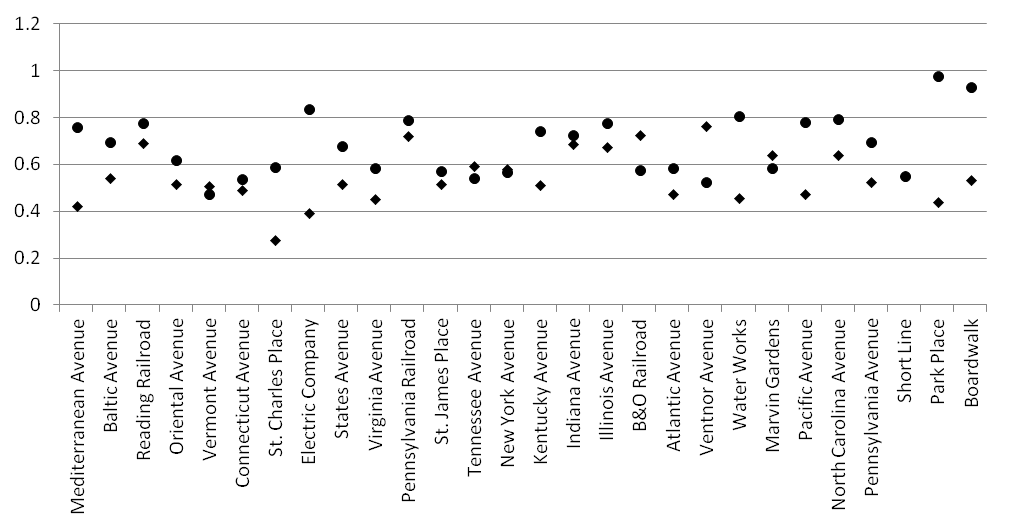
\includegraphics[width=0.75\columnwidth]{Figures/genome.png}}
\caption[Illustration of Genome]{This chart shows part of the genome of the
fittest player in the last generation. This chart compares the chromosome used
when the player already owns a property in the group (represented by the circle
symbol) against the chromosome used when two other players own a property in the
group (the diamond symbol). These two genes show agreement with the heuristic
strategy: the player is more likely to buy a property when there is a chance of
gaining a monopoly, and less likely to buy a property when other players are
blocking the group from being monopolized.}
\label{figure-genome}
\end{figure}

When compared to the strategy list from~\ref{m_gamestrategies}, there might
appear to be an inconsistency in the genome. For example, the strategy says
always buy a property if no one else owns it. However, only the gene value for
Park Place approaches a probability of 1.0 which is implied by the strategy.
This can easily be explained by the fact that if the player declines a property
with probability p, the probability of subsequently buying the property is
higher. This is because when a player declines a property, it is then auctioned
to any player including the declining player. Since the declining player makes
the bid decision based on the same chromosome, the probability of buying the
property then becomes

That is, for the player to not obtain a property requires the player to decline
to buy it twice (the second decline being the loss of the auction). Since these
are independent events, the probability of losing an auction is approximately
\(P_{decline} * P_{decline}\). The probability of obtaining a property is 1
minus that product. Thus, even when the probability of buying is as low as 0.6,
the probability of declining is 0.4, and the probability of obtaining the
property becomes 0.84.

\section{SGA Player}

After evolving the population of RGA Players, the simulation was conducted again
using SGA Players. SGA players are those players with a binary string
chromosome.

The fitness distribution in the first generation shows the same general
similarity to the binomial distribution (Figure~\ref{figure-sga_gen0}), although
there appears to be a bit of skewness.

\begin{figure}[htp]
\centerline{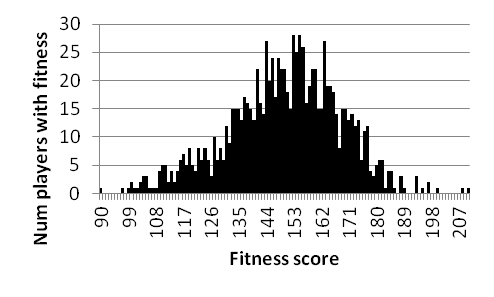
\includegraphics[width=0.75\columnwidth]{Figures/sga_gen0.png}}
\caption[SGA Fitness Generation 0]{This chart shows the actual fitness
distribution for the first generation of an SGA population.}
\label{figure-sga_gen0}
\end{figure}

Figure~\ref{figure-sga_gen289} shows the fitness distribution at generation 289
and the skew is definitely present. It is unclear why this would have occurred.

\begin{figure}[htp]
\centerline{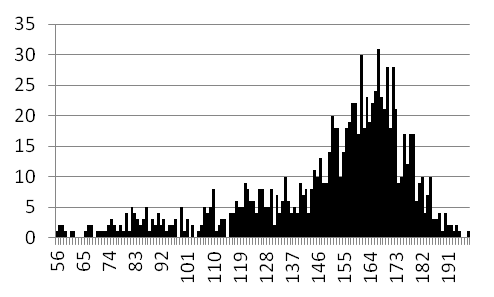
\includegraphics[width=0.75\columnwidth]{Figures/sga_gen289.png}}
\caption[SGA Fitness Generation 289]{This chart shows the actual fitness
distribution for the generation 289 of an SGA population.}
\label{figure-sga_gen289}
\end{figure}

\section{TGA Player}

Finally, the same simulation was conducted using TGA players. The results for
the TGA player were essentially the same as for the RGA player.

The fitness distributions for the initial populations had the same shape as a
binomial distribution, with similar minimums and maximums for the initial
generation as for the RGA chromosomes. Over the 1000 generation simulations, the
fitness distribution converged towards the mean fitness. The minimum, maximum,
mean, and median were essentially the same as the RGA simulation, and the player
genomes were also very similar. This is unsurprising, since the fitness seems to
depend mostly on buying property (in which the RGA and TGA genomes are
identical), and not on getting out of jail which was the difference between the
two genomes.

\section{Validation}

As with other research that used competitive fitness functions, validations of
the various populations were performed to test if the populations were actually
getting better.

\subsection{Intrapopulation validation}

For every population, the best player in the last generation was played against
the best player in generation 250, 500, and 750. 30 games were played with the
same set of 4 best players. If the population was actually evolving better
players, we expect that on average, the best player in the last generation will
win more games then the other players; and the best player in the 250th
generation should lose more games on average. The results are shown in
Figure~\ref{figure-intrapopulation}.

\begin{figure}[htp]
\centerline{
\includegraphics[width=0.75\columnwidth]{Figures/figureTBD.png}}
\caption[Intrapopulation validation]{The results of playing the best player in
the last generation against the best players in previous generations.}
\label{figure-intrapopulation}
\end{figure}

\subsection{Interpopulation validation I}

Next, the best players from the last generation of similar populations that used
different fitness evaluators were played against each other. This was done to
see which, if any, fitness evaluator produced better players. Because of the
highly random nature of the game and based on the previous work comparing
competitive fitness functions, we expected that the TOURNAMENT fitness evaluator
would produce less fit players than at least some of the other fitness
evaluators.

ACTUAL RESULTS TBD. Figure~\ref{figure-interpopulation1} shows the results of
these competitions.

\begin{figure}[htp]
\centerline{
\includegraphics[width=0.75\columnwidth]{Figures/figureTBD.png}}
\caption[Validation - Comparing Fitness Evaluators]{The results of playing the
best player in the last generation against the best players in previous
generations.}
\label{figure-interpopulation1}
\end{figure}

\subsection{Interpopulation validation II}

The best players from the last generation of various populations that used
the same fitness evaluators were also played against each other. This was done
to see if the populations that were smaller could produce comparable
players as the larger populations. As seen in Chapter ~\ref{chap:background},
many previous studies used small populations to produce their results, whereas
the study that this thesis most closely resembles used a poulation of 1000
individuals. For this work, the populations with 1024 individuals took the
longest to evolve. Being able to get comparable results with smaller populations
would be a more efficient use of resources.

ACTUAL RESULTS TBD. Figure~\ref{figure-interpopulation2} shows the results of
these competitions.

\begin{figure}[htp]
\centerline{
\includegraphics[width=0.75\columnwidth]{Figures/figureTBD.png}}
\caption[Validation - Comparing population sizes]{The results of playing the
best player in the last generation against the best players in previous
generations.}
\label{figure-interpopulation2}
\end{figure}
